% Note that the text in the [] brackets is the one that will
% appear in the table of contents, whilst the text in the {}
% brackets will appear in the main thesis.

%% CHAPTER HEADER /////////////////////////////////////////////////////////////////////////////////////
\chapter[Simulation Results and Model Validation]{Simulation Results and Model Validation}
\label{ch:validation}

%% CHAPTER INTRODUCTION ///////////////////////////////////////////////////////////////////////////////
The developed models require validation to assess the accuracy and reliability of the modelled physical processes.
Validation of the \acp{pzt} is performed by analytical analysis of the electromechanical impedance of the circular sensor. 
On the other hand, the \ac{hsc} panel model is evaluated experimentally in two ways: by analysing the full wavefield obtained by the \ac{sldv} and by analysing the time signals measured by the \acp{pzt} setup.
%% INCLUDE SECTIONS ///////////////////////////////////////////////////////////////////////////////////
%% SECTION HEADER /////////////////////////////////////////////////////////////////////////////////////
\section{Validation of the \acs{pzt} model}
\label{sec:pztVal}

%% SECTION CONTENT ////////////////////////////////////////////////////////////////////////////////////
The current model, i.e. the curved boundary geometry approximated with the second-order elements, is validated by comparing the transducer impedance obtained by numerical simulation with (i) analytical model and (ii) experimental results.

The impedance Z is a ratio between voltage \((\Phi)\) and current \((I)\) defined as follows:
\begin{eqnarray}
	Z = \frac{\Phi}{I} = \frac{\Phi}{i\omega Q},
	\label{eq:impedance}
\end{eqnarray}
\nomtypeG[omega_ang]{\(\omega\)}{Angular frequency}{\(2\pi f_c\)}{\unit[per-mode = symbol]{\radian\per\second}}%
\nomtypeR[I]{\(I\)}{Electric current}{-}{\unit{\ampere}}%
\nomtypeD[i]{\(i\)}{Imaginary number}{\(sqrt{-1})\)}%
\nomtypeR[z_impedance]{\(Z\)}{Impedance}{\(\Phi/I\)}{\unit{\ohm}}%
where \(i=\sqrt{-1}\), \(\omega\) is the angular frequency.
In the case of numerical simulation, \(\Phi\) is assumed as the 1.5-cycle Hann windowed sine pulse at carrier frequency 150 \unit{\kHz}, and \(Q\) is the charge induced on the electrode calculated by Eq. (\ref{eq:pzt_sem}).
The excitation signal has significant values in the 0-300 \unit{\kHz} frequency range, as shown in Fig.~\ref{fig:impedance}(\textbf{a}).
The analytical model derived by Giurgiutiu \cite{giurgiutiu2009micromechatronics} is defined as:
\begin{eqnarray}
	Z = \frac{1}{i\omega C_0}\left[\left(1-k_p^2\right)+k_p^2\frac{u_r}{u_I}\right],
\end{eqnarray}
\nomtypeR[Capaci]{\(C_0\)}{Transducer free capacitance}{-}{\unit{\farad}}%
\nomtypeD[kp]{\(k_p\)}{Transducer planar coupling coefficient}{-}%
where \(C_0\) is the free capacitance of the sensor, \(k_p\) is the planar coupling coefficient, \(u_r\) is the displacement response, and \(u_I\) is the induced displacement.
Additionally, for comparison, the response of the \ac{sem} with curved boundary approximated by linear elements was included.
All models refer to the free transducer shown in Fig. \ref{fig:hioki}\textbf{(a)}, i.e. soldered wires and thin electrode coatings have been omitted.

\begin{figure}[H]
	\begin{center}
		\includegraphics[width=0.95\textwidth]{Chapter_6/hioki}
	\end{center}
	\caption{Setup to impedance measurement, \textbf{(a)} Hioki impedance analyser, \textbf{(b)} free \ac{pzt}, \textbf{(c)} transducer with soldered wires ready for measurements.}
	\label{fig:hioki}
\end{figure}
For experimental validation, an impedance analyzer (Hioki, IM 3570) was used to determine the electric current flowing through the transducer under the influence of applied voltage in the form of a sine signal with a variable frequency in the range of 1-300 \unit{\kHz}.
Both characteristics are used to determine the impedance according to Eq. \ref{eq:impedance}.
The measurements were taken at room temperature and averaged 50 times to improve the signal-to-noise ratio.

\begin{figure}[H]
	\begin{center}
		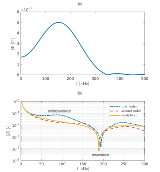
\includegraphics[width=0.95\textwidth]{Chapter_6/impedance}
	\end{center}
	\caption{Validation of the \acf{pzt} model (\textbf{a}) the frequency spectrum of the excitation signal, (\textbf{b}) impedance response of the transducer for numerical model with first order approximation of the boundary dash-dot line, numerical model with second order approximation of the curved boundary dashed line, analytical model dotted line and experimental measurements solid line.}
	\label{fig:impedance}
\end{figure}

It can be notice in Fig.~\ref{fig:impedance}(\textbf{b}) that the impedance of the model with second order approximation elements is in very good agreement with the analytical solution and to experimental results to the resonance peak.
The resonant peak occurred near 190 \unit{\kHz} for second order model and analytical one and 194 \unit{\kHz} in case of experimental measurement.
The model with a first-order approximation is a better fit for the experiment in frequencies above the resonant peak.
In addition, an additional antiresonance peak occurred around 90 \unit{\kHz}, which was not observed in the previous two models and experimental result.

The discrepancy in impedance based on the models and experiment may be due to uncontrolled ambient condition during the measurements and accuracy of piezo and electromechanical properties provided by the manufacturer. 
Additionally, the models were simplified by excluding the wires and solder unlike the tested transducer shown in Fig. \ref{fig:hioki}\textbf{(b)}.


%% SECTION HEADER /////////////////////////////////////////////////////////////////////////////////////
\section{Experimental Setup Configuration}
\label{sec:setup}

%% SECTION CONTENT ////////////////////////////////////////////////////////////////////////////////////

The presented model was validated with results from two experimental studies.
The first one was performed for determination of the full wavefield of the propagating waves by the \ac{sldv} (Polytec PSV–400).
The second study was performed for wave acquisition by the \ac{pzt} sensor.
The schematic of the experimental setup is shown in Figure~\ref{fig:setup}.
The sample of interest was a not-regular hexagonal aluminium honeycomb bonded to one \ac{cfrp} plate  using the epoxy adhesive (Loctite EA3479B) as shown in Figure~\ref{fig:honeycomb}(\textbf{a}).%PF: label acc. to figure caption.
The subject of the parametric study was the effect of the disbond size on the propagating GW.

\begin{figure}[H]
	%	\begin{center}
	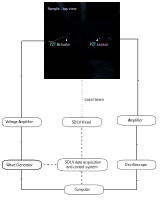
\includegraphics[width=1\linewidth]{Chapter_6/setup}
	%	\end{center}
	\caption{Experimental setup for the (1) \ac{sldv} measurement---dashed line and (2) PZT wave acquisition---solid line.}
	\label{fig:setup}
\end{figure}
\vspace{-12pt}
\begin{figure}[H]
	%	\begin{center}
	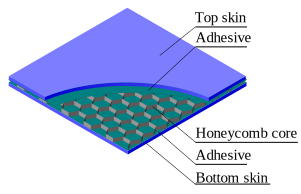
\includegraphics[width=1\linewidth]{Chapter_6/honeycomb}
	%	\end{center}
	\caption{Sample configuration: (\textbf{a}) top view of the sample, (\textbf{b}) honeycomb sandwich substructures and (\textbf{c}) details of the honeycomb cell.}
	\label{fig:honeycomb}
\end{figure}


After a reference measurement was made on an intact sample, several measurements were taken for the subsequent damage introduced on the same specimen.
The circular area of the core was detached from the adhesive at the center of the plate using a sharp hooked tool.
For this purpose, the bottom skin was omitted so that damage could be introduced.
The damage size was controlled by its diameter \(\Phi_D=\left [10, 30, 50, 70, 90, 110, 130 \right ]\) mm.

The generation and reception of elastic waves were achieved with a pair of \ac{pzt} transducers mounted on the skin top surface with the cyanoacrylate glue.
The coordinates of the actuator were \((x_1,y_1)=(-100,0)\) mm,	and for the sensor, \((x_2,y_2)=(100,0)\) mm.
The dimensions of the sample components were as follows:
\begin{itemize}
	\item \ac{cfrp} skin: \(L \times W \times H = 500 \times 500\ \times 1.5\) mm,
	\item Aluminium core: \(g=14.5\) mm, \(w=0.1\) mm, \(h_1=11\) mm, \(h_2=5\) mm, \(l_1=10.4\) mm, \(l_2=6\) mm,
	\item Epoxy adhesive: \(L\times W \times H = 500 \times 500 \times 0.3\) mm,
	\item NCE51 \ac{pzt}: \(\Phi_{PZT}=10\) mm, \(h=0.5\) mm,
	\item Cyanoacrylate glue: \(\Phi_{CG}=10\) mm, \(h=0.05\) mm.
\end{itemize}

The \(N_c=5\) cycle Hann windowed signal at carrier frequencies \mbox{\(f_c=[75,100,125,150]\) kHz} was generated using an arbitrary waveform generator (National Instruments, PXI 5413).
The signal was amplified 40 times and supplied to the \ac{pzt} actuator (Noliac, NCE51).
Each measurement was conducted in the room temperature and averaged 20~times in order to improve the signal to noise ratio.
%% SECTION HEADER /////////////////////////////////////////////////////////////////////////////////////
\section{Results}
\label{sec:resuls}
%% SECTION CONTENT ////////////////////////////////////////////////////////////////////////////////////
\subsection{\acs{hsc} validation with \acs{sldv} setup}
The full wavefield in the reference sample is presented in Fig.~\ref{fig:wavefield}.
The experimental measurements and the \ac{fcgm} snapshots show that the wavefront distortion is rising with the frequency.
Because the wavelength decreases as the frequency increases, a higher frequency signal is more likely to reflect off the core walls.
This effect is not observed in the case of the \ac{hcgm}.
\vspace{-6pt}
\begin{figure}[H]
	\begin{center}
		\includegraphics[width=0.95\textwidth]{Chapter_6/fullfield}
	\end{center}
	\caption{The top surface out of plane particle velocity snapshots in the time 100 \unit{\micro\second} for (\textbf{a}) the experimental results obtained by using the \acf{sldv}, (\textbf{b}) the \acf{fcgm} and (\textbf{c}) the \acf{hcgm} in the healthy~sample.}
	\label{fig:wavefield}
\end{figure}

\begin{figure}[H]
	\begin{center}
		\includegraphics[width=0.95\textwidth]{Chapter_6/fullfield_dam}
	\end{center}
	\caption{The top surface out of plane particle velocity snapshots in the time 100~\unit{\micro\second} for (\textbf{a}) the experimental results obtained by using \ac{sldv} in the sample with 90 \unit{\mm} width damage, (\textbf{b}) the \acf{fcgm} and (\textbf{c}) the \acf{hcgm} with removed core elements in damaged area for both numerical models.}
	\label{fig:wavefield_dam5}
\end{figure}

In case of the damaged sample, the wavefront is not distorted in the damage area bounded by two dotted lines in Fig.~\ref{fig:wavefield_dam5} for all three cases.
Due to the lack of wave leakage into the core, the wave propagates smoothly through the skin.
For the experimental sample and the \ac{fcgm}, interference of waves reflected from the cells and the damage boundary is observed.
The wave interference observed in the \ac{hcgm} refers to waves reflected only from the defect.

\subsection{\acs{hsc} validation with \acsp{pzt} wave acquisition setup}
Validation of the honeycomb structure models and a separate \ac{cfrp} plate intended for the \ac{hsc} sample were done by comparing the group velocity and amplitude of the first packet of \ac{s0} and \ac{a0} arriving at the sensor.
In the Fig.~\ref{fig:signal_exp_raw} are presented examples of the experimentally obtained raw signals for the healthy and damaged samples.
The raw signals are processed for noise reduction and determine an envelope of the signals.
The envelope is used to obtain the amplitude and group velocity of the mods for the model validation and will be used in the analytical assessment of damage magnitude.
\begin{figure}[H]
	\begin{center}
		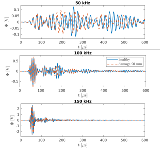
\includegraphics[width=0.95\textwidth]{Chapter_6/signal_exp_raw}
	\end{center}
	\caption{Raw signals registered by the sensor in \acf{hsc} for healthy and damage of 90 \unit{\mm} width.}
	\label{fig:signal_exp_raw}
\end{figure}

Signal processing follows the diagram shown in Fig.~\ref{fig:signal_processing}.
A preliminary step is a conversion of the signals from the time domain to the frequency domain by the \ac{fft}.
Then, the pass-band filter attenuates the frequencies outside of the range \(0.5f_c-1.5f_c\).
A Butterworth filter of 20th order was used.
After filtering the signal is again converted to the time domain by the \ac{ifft}.
Lastly, the envelope of the signal \(e(t)\) is obtained using the Hilbert transform \(\hat{x}(t)\). The definition of both operators given in the book \cite{staszewski2004health} is defined as follows:
\begin{eqnarray}
	\hat{x}(t) &=& \frac{1}{\pi}\int_{-\infty}^{+\infty}x(\tau)\frac{1}{t-\tau}\diff\tau,\\
	e(t) &=& \sqrt{x^2(t)+\hat{x}^2(t)}.
\end{eqnarray}

\begin{figure}[H]
	\begin{center}
		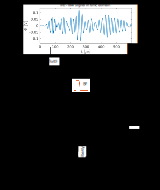
\includegraphics[width=0.95\textwidth]{Chapter_6/signal_processing}
	\end{center}
	\caption{Raw signals registered by the sensor in \acf{hsc} for healthy and damage of 90 \unit{\mm} width.}
	\label{fig:signal_processing}
\end{figure}

The group velocity is derived from the signal envelope determining of the mode \ac{tof}.
The \ac{tof} is a difference between the arrival of the maximum amplitude of the envelope of considered mode at the sensor \((\mathrm{T}_1)\) and the half time of the excitation pulse \(\left(\mathrm{T}_0=\frac{1}{2f_m}\right)\).
Since the distance between the transducers is constant \(l=200\) \unit{\mm}, the group velocity equals:
\begin{eqnarray}
	C_g = \frac{\mathrm{ToF}}{l}=\frac{T_1-T_0}{l}.
\end{eqnarray}
All the experimental signals were processed with the band-pass filter in the frequency range from \(0.5f_c\) to \(1.5f_c\).

The signal envelopes are shown in Fig.~\ref{fig:single_skin} for single \ac{cfrp} plate, Fig.~\ref{fig:hsc_full} for \ac{fcgm}, and Fig.~\ref{fig:hsc_homo}, from which the velocities and amplitudes of the wave mods were determined.
\begin{figure}[H]
	\begin{center}
		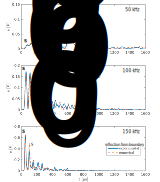
\includegraphics[width=0.95\textwidth]{Chapter_6/single_skin}
	\end{center}
	\caption{The signal envelope for single \acf{cfrp} skin; experimental vs. numerical simulation.}
	\label{fig:single_skin}
\end{figure}
\begin{figure}[H]
	\begin{center}
		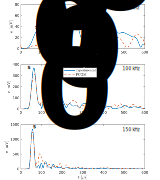
\includegraphics[width=0.95\textwidth]{Chapter_6/HSC_full}
	\end{center}
	\caption{The signal envelope for the \acf{hsc} structure; experimental vs. \acf{fcgm}.}
	\label{fig:hsc_full}
\end{figure}
\begin{figure}[H]
	\begin{center}
		\includegraphics[width=0.95\textwidth]{Chapter_6/HSC_homo}
	\end{center}
	\caption{The signal envelope for the \acf{hsc} structure; experimental vs. the \acf{hcgm}.}
	\label{fig:hsc_homo}
\end{figure}

For the single \ac{cfrp} plate, Tab. \ref{tab:group_velocity_cfrp} gives the determined velocities and amplitudes of the modes together with the percentage errors defined as:
\begin{eqnarray}
	\delta = \left|\frac{x^{num}-x^{exp}}{x^{exp}}\right|\times100\%,
\end{eqnarray}
where \(x^{num}\) and \(x^{exp}\) are the numerical and experimental values, respectively.
It can be noticed that the model are in good agreement with experimental results.
All values are within an error of up to 10\%, except for the \ac{s0} and \ac{a0} amplitudes for 50 and 100 \unit{\kHz}, respectively.
For these cases, the error is about 25\%.
There is no data for the \ac{a0} of 150 \unit{\kHz}, as the high amplitude \ac{s0} reflections mask it.

Regarding the \ac{hsc} panel, best results are achieved for the \ac{fcgm} as it is shown in Tab.~\ref{tab:group_velocity_hsc}.
The velocity error is less then 16.4\% for both modes. 
In the case of amplitude values, only the \ac{s0} of 50 \unit{\kHz} and the \ac{a0} of 100 \unit{\kHz} are overestimated by the model with the error around 25 \%.
For the \ac{hcgm}, best result are obtained for the 100 \unit{\kHz}. 
The velocity error is about 5\% for both modes. 

\begin{table}[H]
	\small
	\tabcolsep=0.2cm
	\centering
	\caption{\label{tab:group_velocity_cfrp} Comparison between of the modes amplitudes and group velocities obtained from the simulations and experiments for the single \acf{cfrp} plate.}
	\begin{tabular}{cccccccc}
		\toprule
		& & \multicolumn{3}{c}{\(C_g\)} & \multicolumn{3}{c}{Amp.}\\
		\multirow{2}{*}{Mode} & Frequency & Exp. & Num. & \(\delta\)& Exp. & Num. & \(\delta\)\\
		& \unit{\kHz} & \unit[per-mode = symbol]{\m\per\s} & \unit[per-mode = symbol]{\m\per\s} & \% & \unit{\mV} & \unit{\mV} & \% \\
		\midrule
		\multirow{3}{*}{\ac{s0}} & 50 & 6079 & 5865 & \textcolor{green}{3.52}& 12 & 171 & \textcolor{red}{25.0} \\
		&100& 5571 & 5747 & \textcolor{green}{3.16} & 171 & 162 & \textcolor{green}{5.26}\\
		&150& 5764 & 5698 & \textcolor{green}{1.15} & 648 & 664 & \textcolor{green}{2.47}\\
		\midrule
		\multirow{3}{*}{\ac{a0}} &50& 1341 & 1325 & \textcolor{green}{0.74} & 134 & 125 & \textcolor{green}{6.72}\\
		&100& 1550 & 1396 & \textcolor{green}{9.74} & 84 & 104 & \textcolor{red}{23.8}\\
		&150& \multicolumn{6}{c}{-} \\
		\bottomrule
	\end{tabular}
\end{table}
\begin{table}[H]
	\small
	\tabcolsep=0.15cm
	\centering
	\caption{\label{tab:group_velocity_hsc} Comparison between of the modes amplitudes and group velocities obtained from the simulations based on \acf{fcgm} and \acf{hcgm} and experiments for \acf{hsc}.}
	\begin{tabular}{cccccccccccc}
		\toprule
		& & \multicolumn{5}{c}{\(C_g\)} & \multicolumn{5}{c}{Amp.}\\
		\multirow{2}{*}{Mode} & Freq.& Exp. & \ac{fcgm} & \(\delta\) & \ac{hcgm} & \(\delta\) &  Exp. & \ac{fcgm} & \(\delta\) & \ac{hcgm} & \(\delta\)\\
		& \unit{\kHz} & \unit[per-mode = symbol]{\m\per\s} & \unit[per-mode = symbol]{\m\per\s} & \% & \unit{\mV} & \unit{\mV} & \% & \unit[per-mode = symbol]{\m\per\s} & \%& \unit[per-mode = symbol]{\m\per\s} & \% \\
		\midrule
		\multirow{3}{*}{\ac{s0}} & 50 & 6329 & 5291 & {16.4} & 8230 & 30 & 33 & 12 & \textcolor{red}{63.6} & 3 & \textcolor{red}{90.9} \\
		&100& 5291 & 5249 & \textcolor{green}{0.79} & 5540 & \textcolor{green}{4.71} & 369 & 341 & \textcolor{green}{7.59} & 152 & \textcolor{red}{58.8}\\
		&150& 5031 & 4866 & \textcolor{green}{2.93} & 4301 & 14.4 & 1340 & 1056 & {21.2} & 359 & \textcolor{red}{73.8} \\
		\midrule
		\multirow{3}{*}{\ac{a0}} & 50 & 964 & 945 & \textcolor{green}{1.97} & 1318 & 36.7 & 62 & 57 & \textcolor{green}{8.06} & 70 & 12.9\\
		& 100 & 2160 & 2075 & \textcolor{green}{3.94} & 2273 & \textcolor{green}{5.23} & 137 & 249 & \textcolor{red}{81.8} & 128 & \textcolor{green}{6.57}\\
		& 150 & \multicolumn{10}{c}{-}\\
		\bottomrule
	\end{tabular}
\end{table}
Errors in the models may be due to several factors.
The most important ones include differences in material properties of used components.
In the models, an average thickness of the adhesive layer was assumed; obtaining precise thickness of the adhesive layer in the specimen preparation is difficult under workshop conditions.
The models also assume a uniform cell geometry for the core area, but in reality, the core is easily deformed in the plane, so the cell geometry varies.
The velocity in the \ac{cfrp} plate varies with the angle of propagation; in the models, the direction of wave propagation between the sensors was assumed to coincide with the plate orientation.
The speed is also affected by the accuracy of the \acp{pzt} placement.
\subsection{Efficiency of the time integration algorithm}
Two types of simulations were conducted to determine the efficiency of the \ac{pa} to solve the equation of motion shown in Section \ref{sec:gpu}.
The first type compares the \ac{pa} computations performed on the \ac{gpu} and \ac{cpu}.
The second type compares \ac{pa} with the benchmark proposed by Kudela et al.~\cite{kudela2020parallel} named \ac{ba}.
Both analyses were performed on the same workstation as the \ac{ba} equipped with the following components:
\begin{itemize}
	\item \ac{cpu} - Intel Xeon Silver, 2.1 \unit{\giga\Hz}, 8 cores
	\item \ac{gpu} - NVIDIA Tesla V100 32 \unit{\giga\byte} 5120 CUDA cores
	\item RAM - 128 \unit{\giga\byte} DDR4 2933 \unit{\mega\Hz}
\end{itemize}

The comparison \ac{gpu} vs. \ac{cpu} was conducted on a \ac{3d} model of an  aluminium plate (\numproduct{250 x250 x 5} \unit{\cubic\mm}).
The structure was discretised with rectangular mesh of the various number of the in-plane elements.
In each case, a spectral element of \numproduct{6 x 6 x 3} nodes with three \acp{dof} per node was used, with one element through the plate thickness.
The global \ac{dof} and the memory usage are presented in Table~\ref{tab:gpuvscpu}.
A concentrated force was applied to the centre of the plate as a 3-cycle Hann windowed sine at 50 \unit{\kHz} frequency.
\begin{table}[!b]
	\tabcolsep=0.2cm
	\centering
	\caption{\label{tab:gpuvscpu} Model parameters used in simulations to compare the algorithm performed on \ac{gpu} and \ac{cpu}.}
	\begin{tabular}{lccccc}
		\toprule
		Number of elements & \numproduct{25 x 25} & \numproduct{50 x 50} & \numproduct{100 x 100} & \numproduct{125 x 125} & \numproduct{250 x 250} \\
		Global \ac{dof}\(\times10^6\) &0.14&0.57&2.26&3.53&14.08\\
		Memory usage \unit{\mega\byte} & 75 & 367 & 1437 & 2252 & 8999\\ \bottomrule
	\end{tabular}
\end{table}
The computational speed up as a function of global \ac{dof} was determined as follows:
\begin{eqnarray}
\mathrm{Speedup} = \frac{\mathrm{CPU_{avg}}}{\mathrm{GPU_{avg}}},
\end{eqnarray}
where \(\mathrm{CPU_{avg}}\) and \(\mathrm{GPU_{avg}}\) is average one time step calculation performed on \ac{cpu} and \ac{gpu}, respectively.
The time of the pre-/post-processing is not included into the speedup calculation, because the data from \ac{cpu} to \ac{gpu} and vice versa is done only once, while the time integration steps are a large number. 

For the second test computations run times of the simulations conducted on \ac{gpu} were computed for various sizes of the composite plate.
The benchmark parameters proposed in the paper mentioned above are gathered in Table~\ref{tab:benchmark}.
The efficiency of the \ac{pa} regarding \ac{ba} is measured by speedup, defined as the ratio of \ac{ba} run time to \ac{pa}.
\begin{table}[!t]
\tabcolsep=0.2cm
\centering
\caption{\label{tab:benchmark}Sample parameters used in the benchmark of the \ac{pa} and the \ac{ba}.}
	\begin{tabular}{lcccccc}
		\toprule
		Plate size \unit{\cm} & \numproduct{30 x 30} & \numproduct{40 x 40} & \numproduct{50 x 50} & \numproduct{70 x 70} & \numproduct{90 x 90} & \numproduct{100 x 100}\\
		Global \ac{dof}\(\times10^6\)&1.02&1.46&1.98&3.09&5.23&6.36\\ \bottomrule
	\end{tabular}
\end{table}

The results of both analysis are pictured in Fig.~\ref{fig:speedup}.
At maximum \ac{dof}, the speedup in \ac{gpu} computation relative to \ac{cpu} computation increases near to 90 and the \ac{pa} is up to ten times more efficient than the \ac{ba}.
Improvement of the algorithm comes from: more operations performed in the preprocessing, transfer of internal forces from the local to the global system by summing columns instead of \verb+for-loop+, and minimized number of columns in the map of local nodes $\textbf{I}_L$ (see section~\ref{sec:gpu}).
\begin{figure}[!tbh]
	\begin{center}
		\includegraphics[width=0.95\textwidth]{Chapter_6/benchmark}
	\end{center}
	\caption{Speedup in function of global \acfp{dof} of the \acf{pa} computation run on \acf{cpu}~vs.~\acf{gpu} dashed line, and compared to \acf{ba} solid line}
	\label{fig:speedup}
\end{figure}

\section{Conclusions}
\label{sec:conclusionsValid}

%% SECTION CONTENT ////////////////////////////////////////////////////////////////////////////////////
This chapter presents the experimental validation of the \ac{fcgm} and \ac{hcgm}.
It is shown that the \ac{fcgm} better expresses the wave propagation in \ac{hsc} than the simplified model.
The snapshots of the full wavefield show wave interference in the core cells, which is impossible in the \ac{hcgm}.
The full-field analysis also showed a lack of wave leakage into the core at the damaged area.
This phenomenon will be the basis for determining the effect of the damage on wave propagation.
The velocity of the wave propagation for both models is in good agreement with the \ac{pzt} measurements.
Additionally, it was shown that by optimising the algorithm for solving the equation of motion, a calculation time was achieved ten times faster than the algorithm presented in the paper \cite{kudela2020parallel}.